\documentclass[../main.tex]{subfiles}
\begin{document}
\section{映射}
\begin{definition}
    设$X$和$Y$是集合,如果由$X$到$Y$的关系$f$同时满足:
    \begin{enumerate}
        \item $\mathrm{dom}f=X$;
        \item 对每一$X$的元素$x\in X$,\emph{有且只有一个}$Y$的元素$y\in Y$满足$\left(x,y\right)\in f$,
    \end{enumerate}
    则称$f$是由$X$到$Y$的\emph{映射(mapping)},记作$f:X\rightarrow Y$\footnote{记号$f:X\rightarrow Y$包含的信息是:
        \begin{enumerate}
            \item $X$、$Y$是集合;
            \item $f$是由$X$到$Y$的映射。
        \end{enumerate}
    }。对每一$\left(x,y\right)\in f$,称$y$是$x$在映射$f$下的\emph{值(value)},记作$f\left(x\right)$。
\end{definition}

\begin{figure}[htbp]
    \centering
    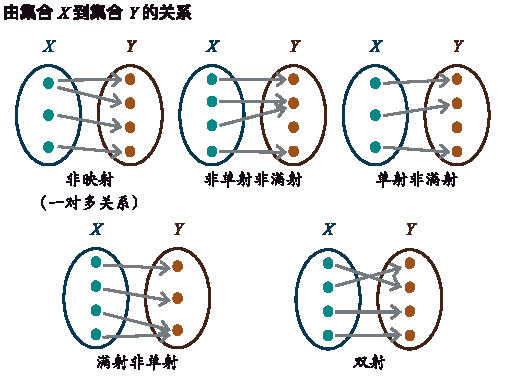
\includegraphics{../images/mapping.pdf}
    \caption{映射的不同概念示意图。}
    \label{fig:II.1.3}
\end{figure}

映射定义的第1条要求如果违反了,可通过对集合$X$的改动重新得到满足,而无需改动关系$f$本身。例如若$\mathrm{dom}f\subsetneqq X$,则令$X^\prime=\mathrm{dom}f$并改为讨论由$X^\prime$到$Y$的关系$f$,就可通过映射定义的第1条。然而映射定义的第2条如果违反了,想要重新满足就不得不对关系$f$本身进行改动。图\ref{fig:II.1.3}中的第一个例子就只是一个关系,而不是一个映射,除非我们从这一关系中拿掉一个有序对。

给定映射$f:X\rightarrow Y$,我们继续以下讨论:
\begin{itemize}
    \item 一般地,$Y$未必等于$\mathrm{ran}f$,集合$Y$称映射$f$的\emph{陪域(codomain)}。
    \item 若$\mathrm{ran}f=Y$则称映射$f$是\emph{满射(surjective mapping)}。图\ref{fig:II.1.3}中的第4和第5个例子都是满射。
    \item 若$A\subset X$,则集合$\left\{y|y\in Y\wedge\left(\forall x\in A,y=f\left(x\right)\right)\right\}$称集合$A$在映射$f$下的\emph{像(image)}。常见但易产生歧义的记法是$f\left(A\right)$。这一集合可用语言描述为:由集合$A$的所有元素在映射$f$下的值组成的集合。易证它是$Y$的子集。
    \item 若对任意$x_1,x_2\in X$,$f\left(x_1\right)=f\left(x_2\right)\Rightarrow x_1=x_2$,则称$f$是\emph{单射(injective mapping)}。可用语言描述为,“单射输出唯一地确定其输入”。图\ref{fig:II.1.3}中的第3和第5个例子都是单射。
    \item 如果$f$既是满射又是单射,则称$f$是一个\emph{双射(bijective mapping)}。图\ref{fig:II.1.3}中的第5个例子是双射。
    \item 若另一映射$g:Y\rightarrow Z$,可与映射$f$构成从$X$到$Z$的映射$g\circ f:X\rightarrow Z$,且
          \[
              g\circ f\left(x\right)=g\left(f\left(x\right)\right),\forall x\in X
          \]
          则称$g\circ f$是$f$和$g$的\emph{复合映射(composite mapping)}。
    \item 如果$f\left(x\right)=x,\forall x\in X$,则称映射$f$是\emph{恒等映射(identity mapping)}。
    \item 如果映射$g:Y\rightarrow X$使得复合映射$g\circ f$是恒等映射,则称映射$f$是\emph{可逆的(invertible)},映射$g$是$f$的\emph{逆映射(inverse mapping)}。常将$f$的逆映射计作$f^{-1}$。
\end{itemize}

关于逆映射,有一条重要的定理——

\begin{theorem}\label{thm:II.1.7}
    双射必存在唯一逆映射。双射的逆映射也是双射。
\end{theorem}
\begin{proof}
    为了证明这一定理,我们首先证明一个引理:任一单射非满射均存在逆映射。

    设$f:X\rightarrow Y$是一个单射非满射,即$\exists y\notin\mathrm{ran}f,y\in Y$。由集合的相关定义此处必有$\left\{y|y\in\mathrm{ran}f\right\}\cup\left\{y|y\notin\mathrm{ran}f,y\in Y\right\}=Y$。

    现定义$g:Y\rightarrow X$,为使$g$为一个映射,它必须对$y\in\mathrm{ran}f$和$y\notin\mathrm{ran}f,y\in Y$均有定义。现将其定义为:
    \[
        g\left(y\right)=\left\{
        \begin{array}{ll}
            \left.x\right|_{f\left(x\right)=y}, & y\in\mathrm{ran}f           \\
            \text{任一}x\in X,                    & y\notin\mathrm{ran}f,y\in Y
        \end{array}
        \right.
    \]
    则有如下几条结论:
    \begin{enumerate}
        \item $g\left(y\right)$是映射。因为它对每一$y\in Y$均有定义且一个$y\in Y$只对应一个$x\in X$。
        \item $g$是满射。因为,仅$y\in\mathrm{ran}f$情况的定义式就已决定了$\mathrm{ran}g=X$。
        \item $g$是非单射。因为$g$是满射,再考虑$y\notin\mathrm{ran}f,y\in Y$情况的定义式,就可知$\exists x\in X$满足$x=g\left(y\right)=g\left(y^\prime\right)$,其中$y\neq y^\prime,y\in\mathrm{ran}f,y^\prime\notin\mathrm{ran}f,y^\prime\in Y$。
        \item $g$是$f$的逆映射。因为,对于任一$x\in X$均有$g\circ f\left(x\right)\equiv g\left(f\left(x\right)\right)=x$,即$g\circ f=\mathrm{id}_X$。
        \item 一般地,$g$是不唯一的。因为$y\notin\mathrm{f},y\in Y$的情况可定义$g\left(x\right)$等于任一$x\in X$,故只要集合$X$不是只有一个元素,那么$g$都不唯一。
    \end{enumerate}
    该引理证毕。

    现在正式证定理\ref{thm:II.1.7}。从上面定义的这个$g$继续,如果$g$是双射,则$g$不仅是满射,还是单射。由刚刚证完的引理,可用类似方法给$g$找一个逆映射$f^\prime:X\rightarrow Y$。而且,由于$\mathrm{ran}g\equiv X$,我们无需像定义$g$那样为$f^\prime$分出$x\notin\mathrm{ran}g,x\in X$的情况,因为不存在这种情况。故
    \[
        f^\prime\left(x\right)=\left.y\right|_{g\left(y\right)=x}
    \]
    是$g$的逆映射,且$f^\prime$是满射。而且,把$g$的定义代入上式有$f^\prime\left(x\right)=\left.y\right|_{g\left(y\right)=x}=\left.y\right|_{\left.x\right|_{f\left(x\right)=y}}=f\left(x\right)$,即$f^\prime$不是别的映射而恰为$f\left(x\right)$。即$g$的逆映射是唯一的。因$f^\prime$是满射故$f$是满射,而$f$本身就是单射,故$f$是双射。
\end{proof}
\end{document}